\begin{figure}[tb]
  % \vspace{-0.7cm}
  \centering
   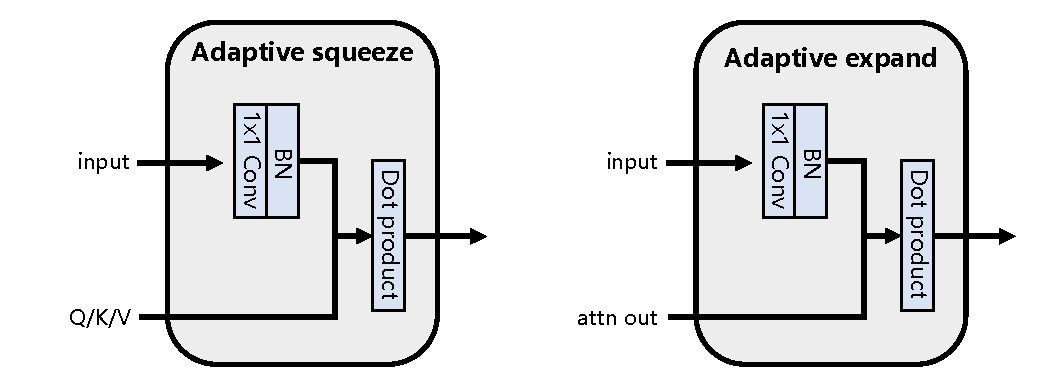
\includegraphics[width=0.8\hsize]{adaptive_sqeeze.pdf}
  \caption{\textit{\textbf{Left}}: the schematic diagram of the proposed adaptive squeezing.
  \textit{\textbf{Right}} is the adaptive expanding operation. \textit{Mat mul} means matrix multiplication. \textit{Attn out} is the output of the multi-head attention.
  }
  \label{fig:squeeze_expand}
  % \vspace{-0.2cm}
\end{figure}